\section{Simulation Setup, Results, and Discussion}
\label{sec:experiments}
\subsection{Simulation Setup}
Thirty fixed tasks cover three scene families, five difficulty levels, and two geometric realizations, denoted A and B. Each level contains six cases, ordered as crossing A/B, passage A/B, and obstacle field A/B. C01--C06 form level 1 and C25--C30 form level 5. These controlled changes test small-team coordination as more routes intersect, shared openings narrow, or obstacle detours grow.
\begin{table}[H]
\caption{Difficulty progression. Each entry has two geometric realizations.\label{tab:cases}}
\small\begin{tabularx}{\textwidth}{lcccccY}
\toprule Family & L1 & L2 & L3 & L4 & L5 & Controlled change \\
\midrule
Crossing & 3 & 4 & 5 & 6 & 7 & Number of UAVs \\
Passage & 4.4 & 4.0 & 3.6 & 3.2 & 2.8 & Square opening width/height (m), $N=5$ \\
Obstacle field & 0.50 & 0.65 & 0.80 & 0.95 & 1.10 & Obstacle half-size multiplier, $N=5$ \\
\bottomrule\end{tabularx}
\end{table}

The common workspace is $[-15,15]\times[-15,15]\times[0.5,7.5]$ m. Crossing tasks connect a perturbed 7 m start ring to opposing goals at radius 4 m, with varied altitudes. Passage and obstacle-field tasks connect starts near $x=-7$ m to assigned goals at $x=4$ m. Their boundary positions and assignments remain fixed across difficulty levels within each realization. The passage wall is 0.7 m thick. The obstacle field contains four boxes, with base half-sizes $(0.35,0.50,0.60)$ m. Fleet growth, opening reduction, and obstacle enlargement provide three distinct difficulty progressions.

The main benchmark uses $T_f=12$ s, $K=60$, and zero initial and final velocities. The common settings are listed in Table~\ref{tab:settings}; the additional stress tests vary one designated parameter at a time. The planner was implemented in MATLAB R2021b using CasADi 3.6.1~\cite{andersson2019} and Ipopt~\cite{wachter2006} with the MA27 linear solver~\cite{hslma27}. Simulations were performed on an Intel Core i9-12900H computer with 16 GB RAM.
\begin{table}[htbp]
\begin{adjustwidth}{-\extralength}{0cm}
\caption{Common physical and numerical settings.\label{tab:settings}}
\small\begin{tabularx}{\fulllength}{lYlY}
\toprule Parameter & Value & Parameter & Value \\
\midrule
Horizon / intervals & 12 s / 60 & Initial / final speed & 0 / 0 m/s \\
Sphere radius $r$ & 0.25 m & Surface clearance $c$ & 0.10 m \\
$v_{\max}$ & 4 m/s & $a_{\max}$ & 3 m/s$^2$ \\
STC / RSTC limits $\ell_s,\ell_r$ & 1.5 / 1.2 m & Expansion step $\Delta_c$ & 0.15 m \\
Geometric guard & $10^{-5}$ m & Control-effort weight & 0.05 \\
Initial / maximum weights & $10^3$ / $10^5$ & Growth factors $\beta_q,\beta_s$ & 2 \\
Defect tolerance $\varepsilon_q$ & $10^{-3}$ m$^2$ & Slack tolerance $\varepsilon_s$ & $10^{-3}$ m \\
Hard-bound tolerance $\varepsilon_h$ & $2\times10^{-5}$ & Maximum outer iterations & 30 \\
Clearance / workspace tolerance & $2\times10^{-5}$ m & Speed tolerance & $2\times10^{-5}$ m/s \\
Acceleration tolerance & $2\times10^{-5}$ m/s$^2$ & Ipopt tolerance & $10^{-6}$ \\
Endpoint / identity tolerance & $10^{-9}$ & Nominal stopping budget & 30 s \\
\bottomrule\end{tabularx}
\end{adjustwidth}
\end{table}

Hard-bound tolerances are applied in native SI units. Endpoint and integration tolerances are $10^{-9}$ m and $10^{-9}$ m/s for position and velocity, respectively.

Reference generation uses a 0.65 m guide grid, a 0.02 s simulation step, and a 2 m/s preferred speed, with the interaction parameters in Table~\ref{tab:initialization}. Arrival thresholds are $\epsilon_p=0.10$ m and $\epsilon_v=0.15$ m/s, and the simulation limit is 30 s. Both reference variants then use the common scalar timing law~\eqref{eq:scalarprofile}.

\begin{table}[htbp]
\caption{Reference-generation parameters.\label{tab:initialization}}
\small\begin{tabularx}{\textwidth}{lYlY}
\toprule Parameter & Value & Parameter & Value \\
\midrule
Look-ahead $\ell_g$ & 0.35 m & Response time $\tau_v$ & 0.3 s \\
Goal time scale $\tau_g$ & 0.6 s & Goal taper distance $d_g$ & 0.75 m \\
Pair gain $A_p$ & 4 m/s$^2$ & Decay length $B_p$ & 0.35 m \\
Interaction buffer $b_p$ & 0.8 m & Pair range $d_{\rm cut}$ & 3 m \\
Tangential factor $\kappa$ & 0.25 & Exponential cap $\chi_{\max}$ & 15 \\
Obstacle gain $A_o$ & 4 m/s$^2$ & Obstacle range $d_o$ & 2 m \\
Boundary buffer $b_w$ & 1.2 m & Zero-distance guard $\epsilon_d$ & $10^{-10}$ m \\
\bottomrule\end{tabularx}
\end{table}

\subsection{Evaluation Protocol and Ablations}
All comparisons preserve the scene, assigned endpoints, flight horizon, motion limits, control-effort objective, and complete-interval acceptance tests. The initialization and recovery ablation comprises three variants:
\begin{enumerate}
\item \textbf{Proposed LIOM}: synchronized A*/SFM geometry, common scalar timing, and the complete two-penalty recovery procedure.
\item \textbf{Straight + LIOM}: straight start--goal geometry with the same scalar timing rule; all subsequent recovery settings are unchanged. It receives no static guide. This variant evaluates the combined contribution of guided reference construction and guide-assisted seed relocation during later corridor updates.
\item \textbf{Hard-once}: the same guided reference, with exact kinematics and hard relative boxes imposed in a single initial-corridor QP.
\end{enumerate}
LIOM allows 200 inner iterations and 5 CPU seconds per solve, capped by the remaining budget. Hard-once receives the remaining budget and up to 6,000 inner iterations. This ablation evaluates the complete recovery mechanism, combining softening, penalty updates, and corridor reconstruction.

The nominal 30 s stopping budget is checked before corridor construction and before assembly and solution. An ongoing solve, reconstruction, and validation finish before the next check, so elapsed time can exceed the nominal budget. Deadline success counts only accepted outputs completed within the stated wall-clock deadline.

The primary metrics are accepted-scene count and CPU time; wall time and deadline success describe elapsed planning performance. Timing includes initialization, construction, solution, and acceptance, with all attempts included and plotting excluded. Each 30-scene comparison is repeated three times with rotated case and method order. Success outcomes agree across repetitions, so counts use 30 distinct scenes. Figure~\ref{fig:performance} reports the three-variant ablation batch. Table~\ref{tab:externalresults} reports the separate paired computational comparison, in which Proposed LIOM and Hard-once are rerun alongside all four additional baselines. Timing comparisons are made within each batch.

\subsection{Trajectory Feasibility}
Complete-interval clearance and motion-limit checks on the reconstructed trajectory~\eqref{eq:arc} determine final acceptance. Every UAV pair and obstacle is included. Squared pair distance is quartic in interval time; its stationary points follow from a cubic polynomial. For point-to-AABB distance, intervals are split at box-face crossings, and the piecewise quartic distance is minimized over endpoints and stationary points. Workspace extrema, fixed endpoint states, and both discrete integration identities are also checked. Final acceptance enforces both the Euclidean limits $v_{\max},a_{\max}$ and the conservative componentwise limits $v_c,a_c$. Velocity is affine within each interval, so its Euclidean norm and each absolute component attain their maxima at interval endpoints; acceleration is constant on that interval. These checks cover each complete flight interval.

Table~\ref{tab:verification} summarizes all 883 accepted runs across the ablations, computational comparisons, and pressure tests. Integration errors measure consistency of the returned representation; clearance and motion-limit checks establish acceptance under the planning model. Nodal displacement is measured from the optimizer's position variables to the final integrated output, including both integration and control correction.
\begin{table}[htbp]
\caption{Output consistency and clearance over all 883 accepted runs in the ablation, computational comparison, and pressure tests. Errors, control corrections, and nodal displacements are maximum absolute component values.\label{tab:verification}}
\small\begin{tabularx}{\textwidth}{Yr}
\toprule Quantity & Observed value \\
\midrule
Position integration error (m) & $8.882\times10^{-16}$ \\
Velocity integration error (m/s) & $2.220\times10^{-16}$ \\
Endpoint-position error (m) & $1.732\times10^{-14}$ \\
Endpoint-velocity error (m/s) & $1.834\times10^{-15}$ \\
Minimum pair center distance (required: 0.60 m) & 0.7215 m \\
Minimum obstacle surface clearance (required: 0.10 m) & 0.1986 m \\
Maximum control correction & $1.521\times10^{-5}$ m/s$^2$ \\
Maximum nodal displacement from optimizer output & $1.286\times10^{-2}$ m \\
\bottomrule\end{tabularx}
\end{table}


\subsection{Cooperative Motions and Reference Timing}
Figure~\ref{fig:allcases} presents the cooperative trajectories for all 30 cases. Figure~\ref{fig:scenes} enlarges the first realization at the highest difficulty level in each family, with two viewpoints per case. Colors identify UAVs within a case, circles mark starts, and triangles mark fixed goals.
\begin{figure}[p]
\begin{adjustwidth}{-\extralength}{0cm}
\centering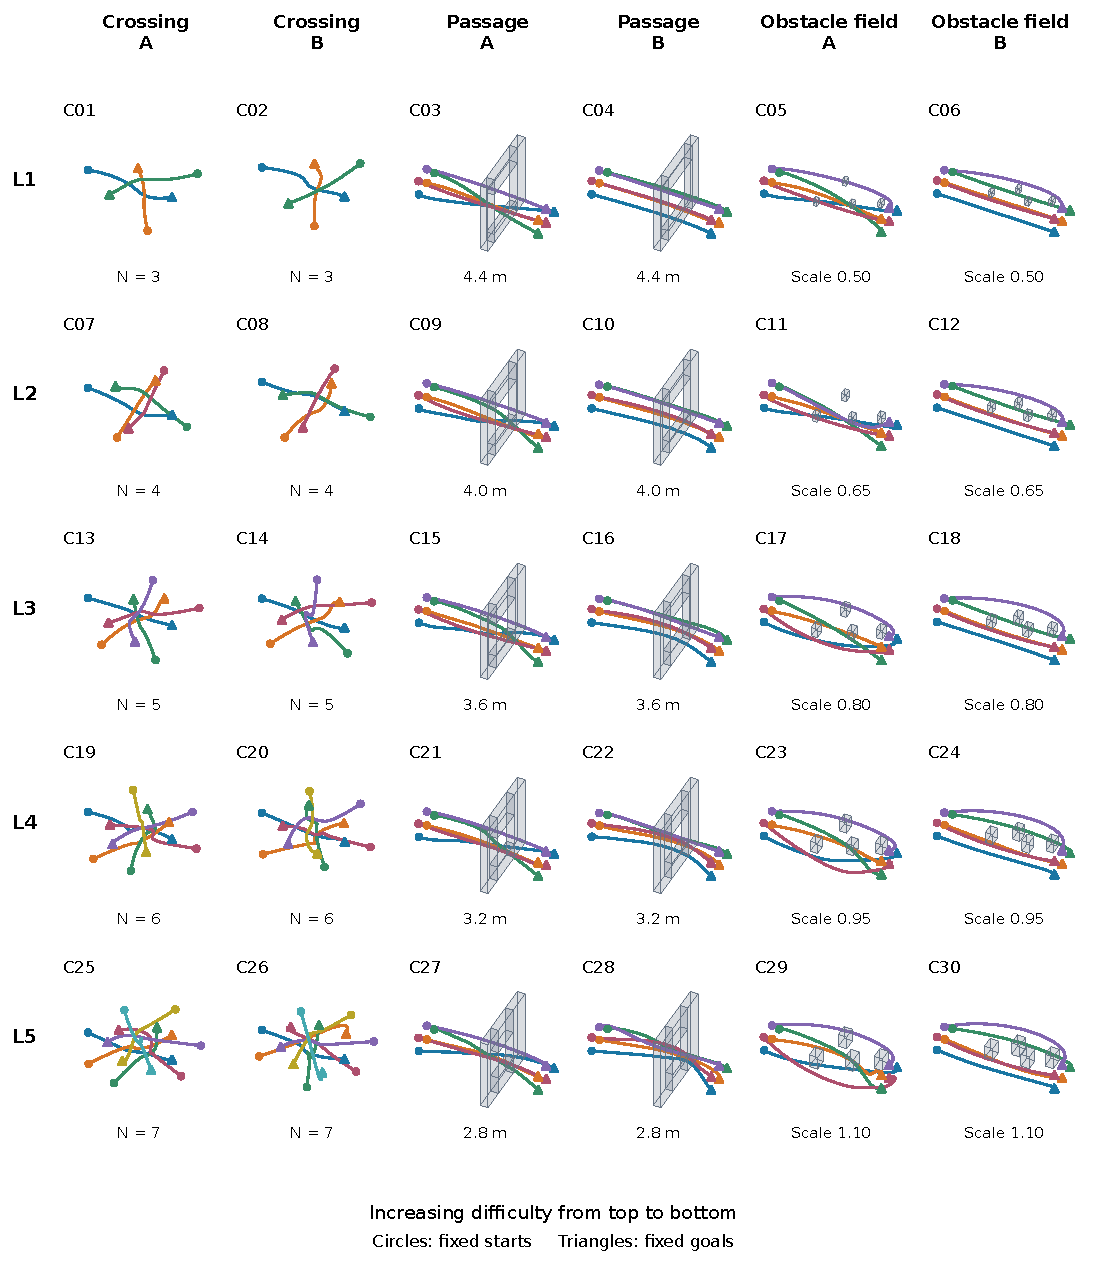
\includegraphics[width=\fulllength,height=20.6cm,keepaspectratio]{figures_rest/all_cases.pdf}
\caption{All 30 rest-to-rest cooperative motions. Rows indicate increasing difficulty; paired columns show the two realizations of each scene family. Small-panel axis ticks are omitted; metric enlarged views appear in Figure~\ref{fig:scenes}.\label{fig:allcases}}
\end{adjustwidth}
\end{figure}
\begin{figure}[p]
\begin{adjustwidth}{-\extralength}{0cm}
\centering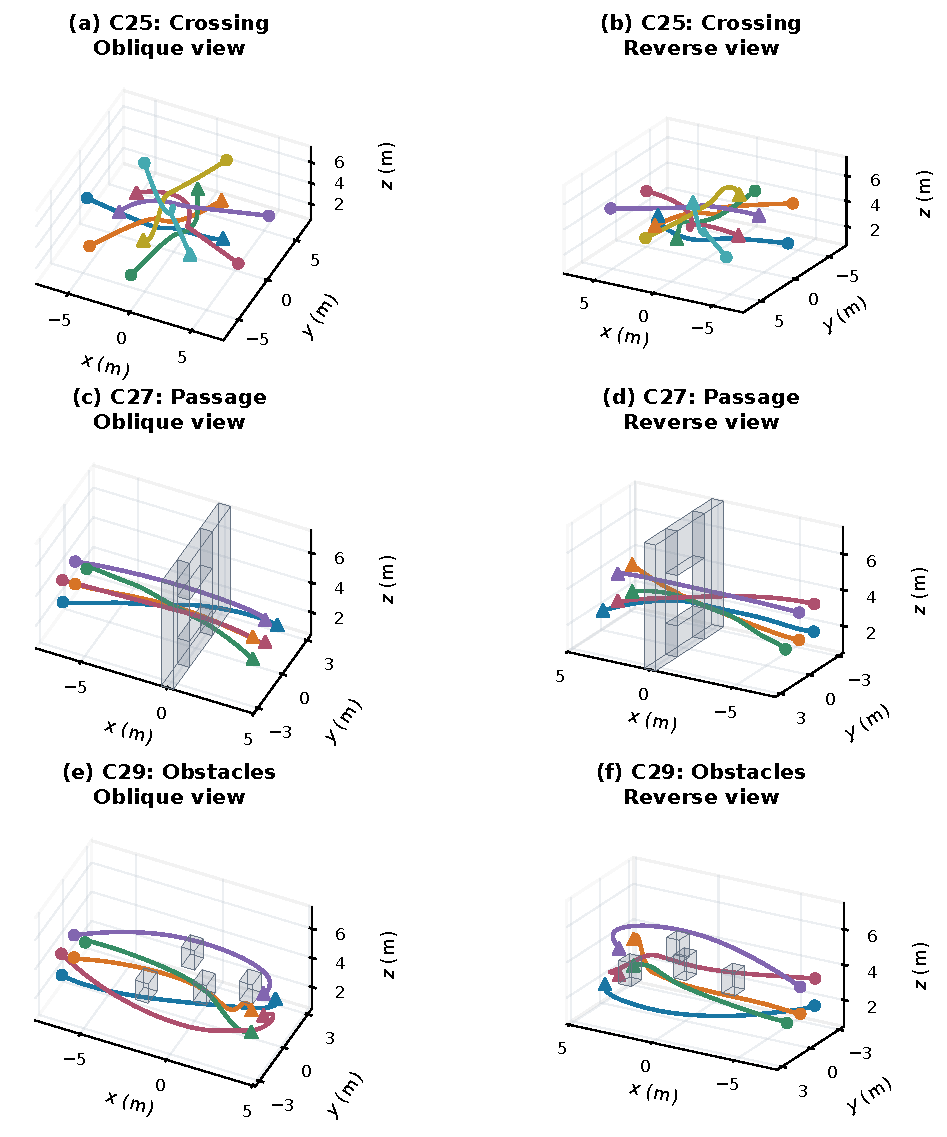
\includegraphics[width=\fulllength,height=20cm,keepaspectratio]{figures_rest/scene_families.pdf}
\caption{Three level-5 examples, each shown from an oblique and reverse view: C25, seven-UAV crossing; C27, five-UAV passage through a 2.8 m opening; and C29, the enlarged obstacle field. Obstacle surfaces are clipped to the displayed window; full geometry is used for planning and checking.\label{fig:scenes}}
\end{adjustwidth}
\end{figure}

C27 illustrates how the spatial reference and final motion differ while maintaining the same task boundaries. Figure~\ref{fig:passage} shows the reference and returned trajectories from an identical camera and gives two orthogonal projections. A projected overlap does not imply a simultaneous three-dimensional collision. Figure~\ref{fig:controls} shows the corresponding continuous velocities and piecewise-constant acceleration controls for all five UAVs.
\begin{figure}[!htb]
\begin{adjustwidth}{-\extralength}{0cm}
\centering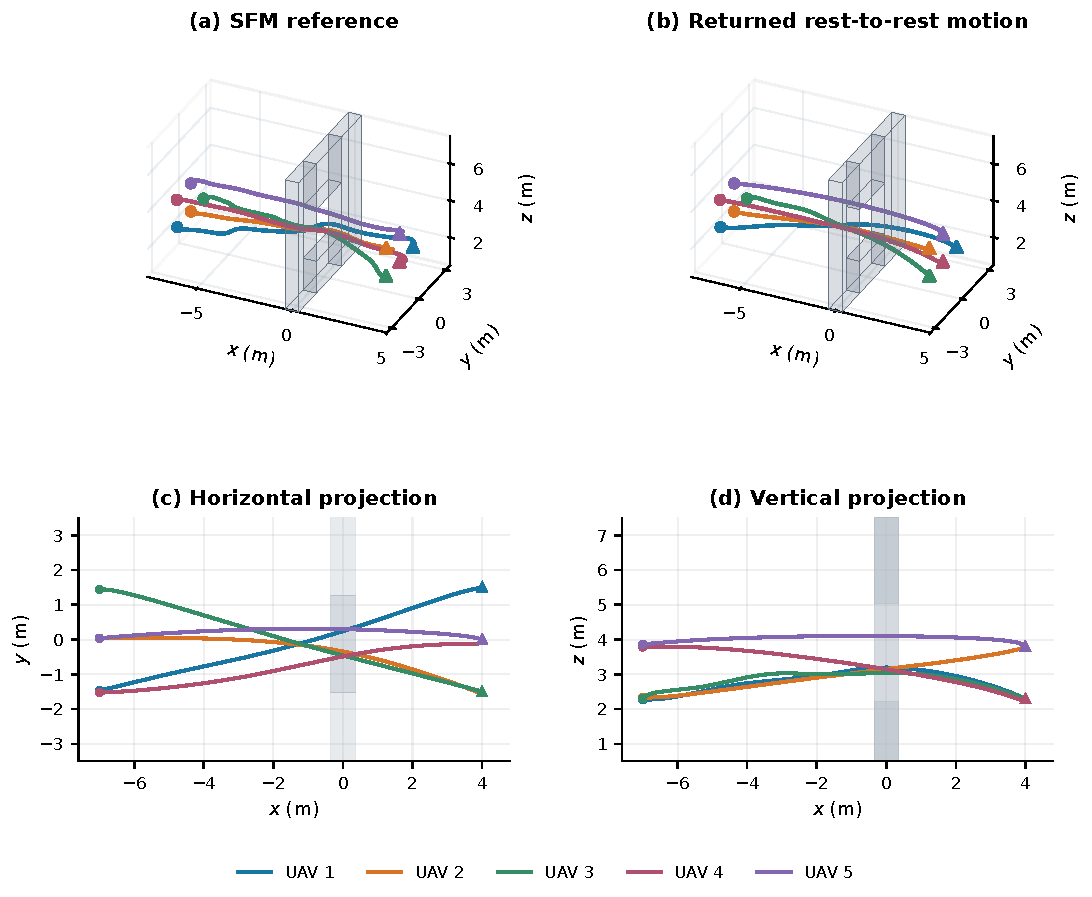
\includegraphics[width=\fulllength]{figures_rest/passage_motion.pdf}
\caption{C27 reference and returned motion, followed by horizontal and vertical projections. Both reference and output have a 12 s horizon and fixed start--goal assignments. Gray planar regions are obstacle projections.\label{fig:passage}}
\end{adjustwidth}
\end{figure}
\begin{figure}[htbp]
\begin{adjustwidth}{-\extralength}{0cm}
\centering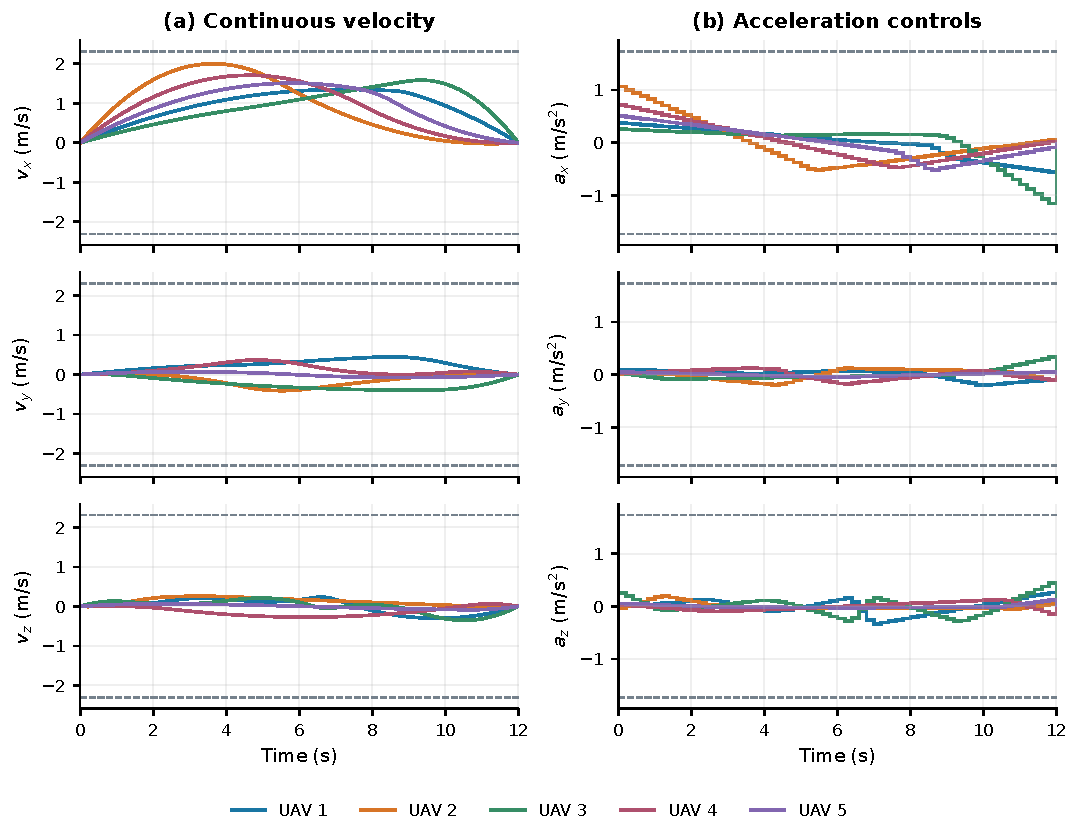
\includegraphics[width=\fulllength]{figures_rest/passage_controls.pdf}
\caption{C27 states and controls. Every velocity curve is continuous and begins and ends at zero. Acceleration is constant on each interval. Dashed lines mark the conservative Cartesian bounds.\label{fig:controls}}
\end{adjustwidth}
\end{figure}

\begin{samepage}
The timing comparison in Figure~\ref{fig:profiles} uses the same admissible scalar rule for SFM and straight geometry. Profile amplitudes depend on their joint path lengths. The common horizon and endpoint-speed conditions provide a consistent timing basis for comparing the two geometric initializations.
\par\end{samepage}
\begin{figure}[htbp]
\begin{adjustwidth}{-\extralength}{0cm}
\centering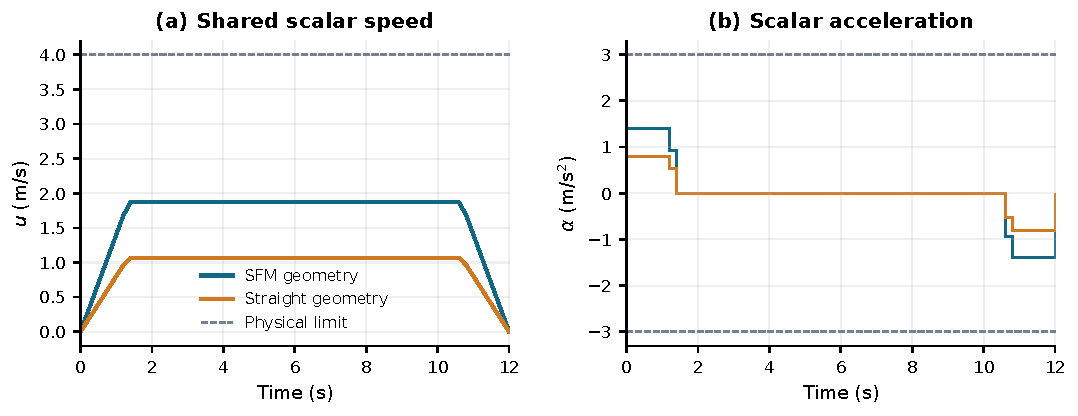
\includegraphics[width=\fulllength]{figures_rest/reference_profiles.pdf}
\caption{C27 scalar reference timing for the two geometric initializations. Both use the same scaled trapezoidal law, prescribed horizon, and zero boundary speeds; dashed lines show the common physical limits.\label{fig:profiles}}
\end{adjustwidth}
\end{figure}

\subsection{Initialization and Recovery Ablations}
Proposed LIOM accepts 30/30 scenes, Straight + LIOM accepts 7/30, and Hard-once accepts 29/30. Figure~\ref{fig:performance} relates these outcomes to per-case CPU time and wall-clock deadlines. Guided reference construction and subsequent guide availability supply useful static detours and passing patterns, increasing success and reducing computation relative to the straight-reference variant. The one-shot formulation is efficient on compatible initial corridors; Proposed LIOM additionally accepts C26 after a second solve.
\begin{figure}[htbp]
\begin{adjustwidth}{-\extralength}{0cm}
\centering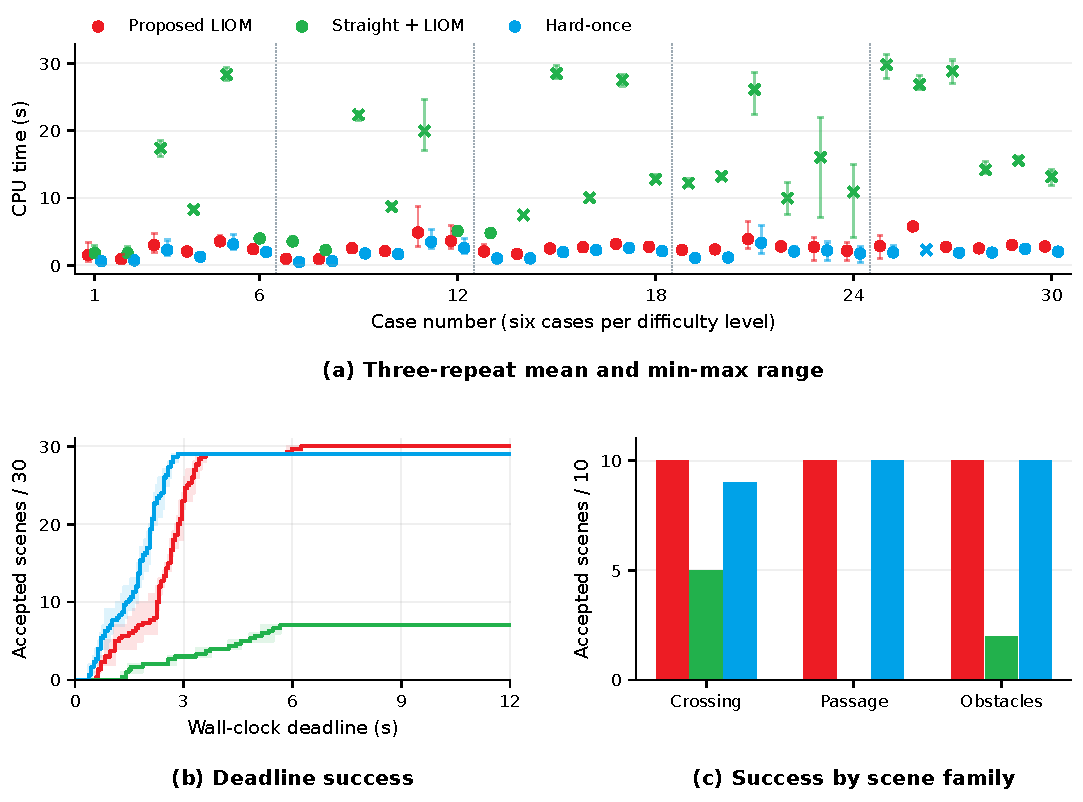
\includegraphics[width=\fulllength]{figures_rest/performance.pdf}
\caption{Initialization and recovery ablation batch. (a) Per-case CPU means and min--max ranges over three repetitions; circles mark acceptance and crosses failure. (b) Accepted scenes by wall-clock deadline, with repetition ranges shaded. (c) Scene-family acceptance. Failed attempts remain in timing statistics.\label{fig:performance}}
\end{adjustwidth}
\end{figure}

The flight duration is fixed at 12 s for every variant. The computation shown in Figure~\ref{fig:performance} precedes execution of that motion.

\subsection{Recovery from Incompatible Initial Corridors}
Proposed LIOM accepts 29 main-benchmark cases after one solve and C26 after two. In C26, the first solve gives $D=1.36\times10^{-2}$ m$^2$ and $S=2.85\times10^{-2}$ m. Both exceed their recovery thresholds. After the weights increase to 2,000 and the corridors are rebuilt, the second candidate reaches $D=4.85\times10^{-9}$ m$^2$ and $S=7.91\times10^{-11}$ m; its reconstructed motion passes the complete-interval checks.

\begin{samepage}
C26's initial hard-box infeasibility was independently confirmed with HiGHS~\cite{huangfu2018}. For the row-scaled linear system $Ax\leq b$, a Phase-I program gives a minimum common relaxation of $1.5175\times10^{-2}$. Nonnegative dual multipliers satisfy $\|A^\top y\|_\infty=2.08\times10^{-17}$ and $b^\top y=-1.5175\times10^{-2}$, with a positive contradiction margin after accounting for finite state bounds. This numerical certificate concerns the selected initial boxes. The accepted second-round trajectory demonstrates recovery of the unchanged physical task through revised local geometry.
\par\end{samepage}

Together, the ablations show the roles of a coordinated reference and the complete recovery procedure. The pressure tests below examine the latter across multiple layouts and degrees of local restriction.

\subsection{Task-Matched Computational Comparison}
\label{sec:external}
Four computational baselines use the common guided reference, hard integration equations, and the same physical task and acceptance tests:
\begin{samepage}
\begin{itemize}
\item \textbf{ASCO-3D}: adaptive risk-range selection of nonlinear collision constraints~\cite{li2021asco}, with range contraction after failed reduced solves and expansion after full-check violations.
\item \textbf{Hard RSC-QP}: spatial boxes and hard relative separating half-spaces based on the relative safe flight corridor principle~\cite{park2021}. This fixed-horizon, centralized variant isolates the hard-corridor component; the cited online planner additionally uses slack and reciprocal avoidance.
\item \textbf{SCP-3D}: successive affine lower bounds on squared separation distances~\cite{augugliaro2012}.
\item \textbf{Direct NLP}: simultaneous enforcement of all nonlinear distance constraints in one solve.
\end{itemize}
\par\end{samepage}
For a reference relative position $\mathbf r^0$ and padded separation $R$, the two affine representations are
\begin{equation}
 \underbrace{\frac{(\mathbf r^0)^\top\mathbf r}{\norm{\mathbf r^0}_2}\geq R}_{\text{Hard RSC-QP}},\qquad
 \underbrace{2(\mathbf r^0)^\top\mathbf r\geq R^2+\norm{\mathbf r^0}_2^2}_{\text{SCP-3D}}.
 \label{eq:baseline-separation}
\end{equation}
Hard RSC-QP uses padded nodes and the common spatial boxes. The other baselines use quarter-interval samples, reachable-displacement padding over $h/8$, and spherical-UAV/AABB distances or their linearizations. Signed distance preserves a penetration gradient for nonlinear intermediate candidates. Each accepted output undergoes the same complete-interval check. These choices compare local constraint representations under identical endpoints, motion limits, and flight duration.

All baselines use the nominal 30 s budget and up to 6,000 inner iterations per solve. ASCO-3D limits each reduced solve to 5 CPU seconds; the others receive the remaining budget. Iterative strategies allow at most 30 solves. ASCO's risk-range parameters are scaled by the ratio of UAV radius to the original covering-disc radius and remain fixed across scenes. Three paired batches rerun Proposed LIOM and Hard-once alongside the four baselines.

\begin{table}[htbp]
\begin{adjustwidth}{-\extralength}{0cm}
\caption{Paired computational comparison on the 30 main-benchmark scenes. Proposed LIOM is the complete method developed in this paper.\label{tab:externalresults}}
\small\setlength{\tabcolsep}{4pt}
\begin{tabularx}{\fulllength}{Yrrrrr}
\toprule Method & Accepted & Within 30 s & CPU mean (s) & Wall mean (s) & Wall P95 (s) \\
\midrule
\textbf{Proposed LIOM} & 30/30 & 30/30 & $1.44\pm0.43$ & $1.31\pm0.40$ & 3.03 \\
Hard-once & 29/30 & 29/30 & $0.92\pm0.31$ & $0.82\pm0.30$ & 2.45 \\
ASCO-3D & 30/30 & 30/30 & $2.14\pm0.53$ & $2.12\pm0.59$ & 6.74 \\
Hard RSC-QP & 30/30 & 30/30 & $1.01\pm0.26$ & $0.91\pm0.25$ & 2.48 \\
SCP-3D & 30/30 & 30/30 & $2.09\pm0.45$ & $2.02\pm0.48$ & 4.87 \\
Direct NLP & 30/30 & 23--29/30 & $11.38\pm2.34$ & $12.01\pm2.75$ & 31.70 \\
\bottomrule\end{tabularx}
\par\vspace{3pt}\footnotesize Counts refer to 30 distinct scenes. The deadline column gives the range across three repetitions; accepted counts are identical in all repetitions. Timing includes every attempt. $\pm$ denotes the SD of the three batch means; P95 uses all 90 attempts per method.

\end{adjustwidth}
\end{table}

Table~\ref{tab:externalresults} shows that Proposed LIOM accepts all scenes at a mean CPU time of 1.44 s, below ASCO-3D, SCP-3D, and Direct NLP. The accepted outputs also meet the 30 s deadline in every repetition. ASCO's constraint selection reduces the cost of the all-distance nonlinear formulation, while the corridor and affine-separation methods exploit the quadratic structure of fixed-horizon translational planning.

Hard RSC-QP accepts all 30 scenes at a mean wall time of 0.91 s, compared with 1.31 s for Proposed LIOM. It also accepts C26 using its initial half-spaces, illustrating how a different local region can resolve a particular incompatibility before iteration begins. The pressure tests examine the complementary requirement: continuing refinement when the local region conflicts with the fixed-horizon task.

The deadline column separates accepted motion from timely completion. Direct NLP returns accepted outputs for all scenes, with 29, 29, and 23 completed within 30 s across the three repetitions; its wall-time P95 is 31.70 s. The remaining methods' accepted main-benchmark outputs finish within 30 s.

\subsection{Recovery under Time and Corridor Pressure}
\label{sec:stress}
The pressure tests use the five-, six-, and seven-UAV crossing layouts C13/C14, C19/C20, and C25/C26. One sweep varies $T_f$ from 8 to 12 s; the other fixes $T_f=12$ s and varies the spatial-box face-growth cap $\ell_s$ from 0.15 to 1.50 m. Both retain $K=60$ and the common physical limits. Each sweep contains 30 settings across six base layouts, with six shared default settings. The growth cap controls local corridor freedom; physical obstacle geometry is unchanged. Proposed LIOM, Hard-once, and Hard RSC-QP use the same cap in each setting, and all failed attempts remain in the counts.

\begin{table}[htbp]
\begin{adjustwidth}{-\extralength}{0cm}
\caption{Acceptance under time and spatial-corridor pressure. Each sweep contains 30 parameter settings across six base layouts.\label{tab:stresssummary}}
\small\begin{tabularx}{\fulllength}{Yrrr}
\toprule Sweep & \textbf{Proposed LIOM} & Hard-once & Hard RSC-QP \\
\midrule
Flight horizon, 8--12 s & 27/30 & 20/30 & 26/30 \\
Spatial-box growth cap, 0.15--1.50 m & 30/30 & 20/30 & 25/30 \\
\bottomrule\end{tabularx}
\end{adjustwidth}
\end{table}


Table~\ref{tab:stresssummary} summarizes acceptance, and Figure~\ref{fig:pressure} locates the recovered settings. In the time sweep, Proposed LIOM accepts 27/30, Hard-once 20/30, and Hard RSC-QP 26/30. Proposed LIOM recovers seven Hard-once failures across four layouts; independent feasibility checks confirm initial hard-box incompatibility in all seven. Nine accepted settings require multiple solves, with at most five. Compared with Hard RSC-QP, the proposed method additionally accepts the six-UAV B and seven-UAV A layouts at 8 s, while Hard RSC-QP alone accepts seven-UAV B at 10 s.

\begin{figure}[!htb]
\begin{adjustwidth}{-\extralength}{0cm}
\centering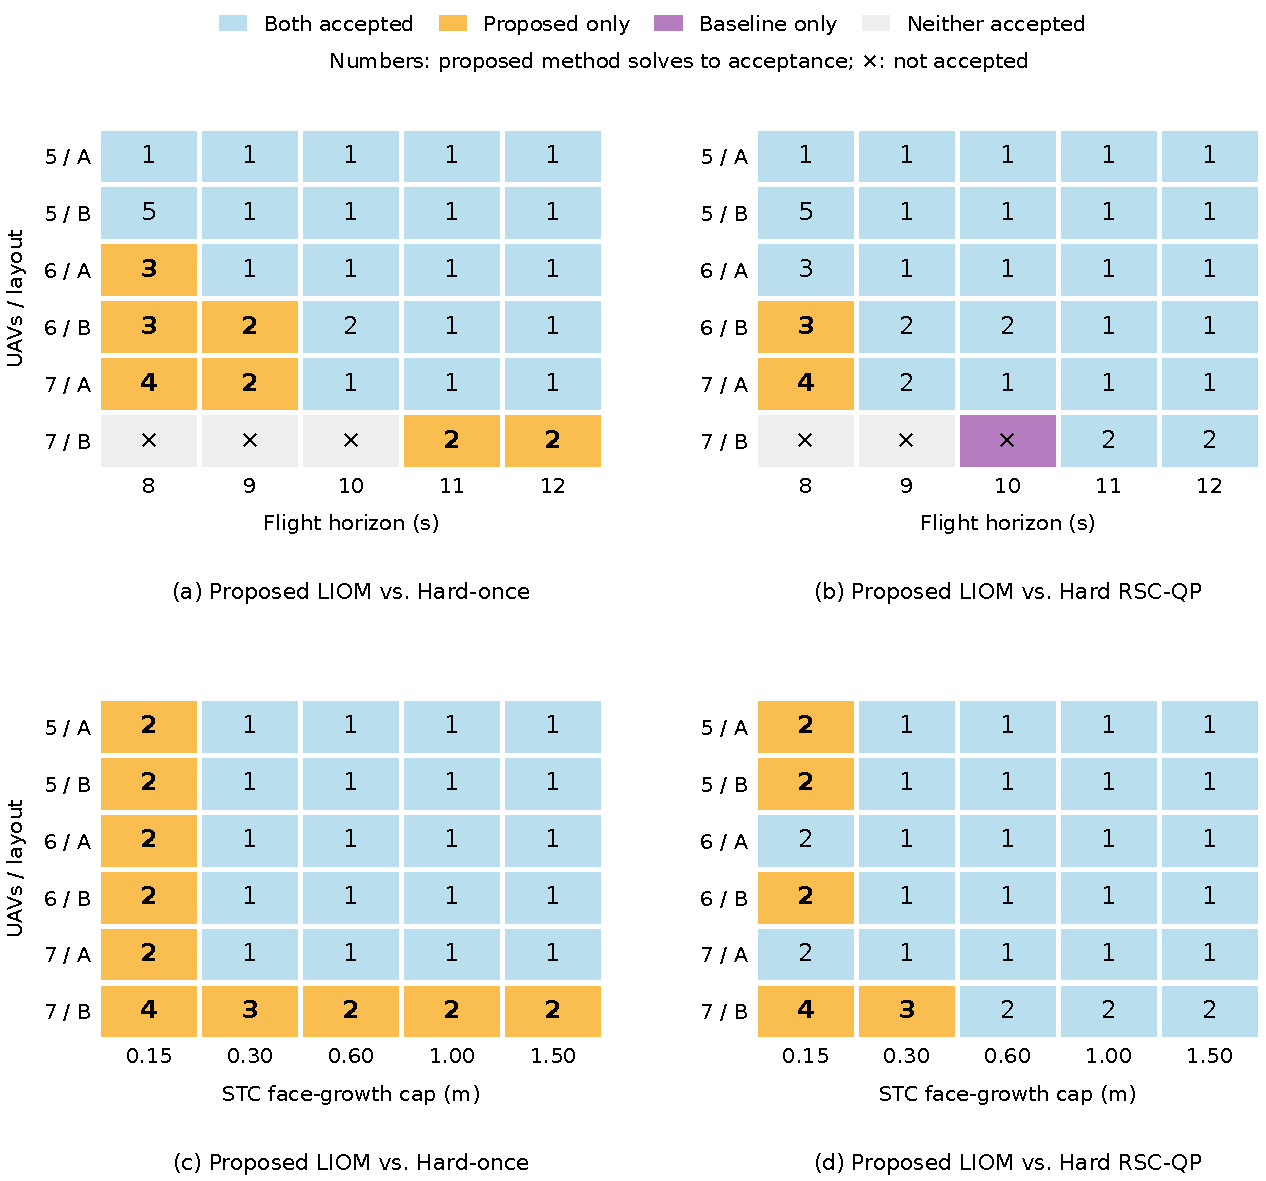
\includegraphics[width=\fulllength]{figures_rest/pressure_sweep.pdf}
\caption{Acceptance across the pressure grids. The upper row varies flight time; the lower row varies spatial-box freedom. A/B denote the two geometric realizations. Colors compare Proposed LIOM with each indicated baseline. Numbers give the proposed method's solves to acceptance; a cross marks its unaccepted attempt.\label{fig:pressure}}
\end{adjustwidth}
\end{figure}

The spatial-box sweep more clearly separates the methods: Proposed LIOM accepts 30/30 settings, Hard-once 20/30, and Hard RSC-QP 25/30. Ten settings have independently confirmed infeasible initial hard-box problems and are recovered in two to four solves. At the smallest cap, every layout requires recovery. All five Hard RSC-QP failures are accepted by the proposed method. Once a hard local region excludes the admissible motion, the low cost of its QP alone offers no route forward. The proposed procedure instead uses intermediate candidates to relocate the corridors while preserving flight time, endpoints, and physical bounds.

The maximum observed wall times among accepted Proposed LIOM runs are 8.51 s in the time sweep and 2.03 s in the box sweep. The seven-UAV B reference exceeds the scalar timing limit at 8 s; at 9 and 10 s, numerical recovery is reached, but the reconstructed outputs do not pass the componentwise motion checks within the stopping budget.

Together, the sweeps demonstrate recovery across multiple layouts and degrees of local restriction. Compatible initial geometry permits a short hard-corridor solve. When that compatibility is lost, the complete recovery procedure provides intermediate candidates for geometry updates and subsequent acceptance at the unchanged flight horizon.

